%%%%% Techinical Preliminaries %%%%%

In this section I will give an overview of
mathematical and computational concepts
that I will use throughout the rest of this document. 
First, since I consider preference relations that are modeled
as binary relations,
I recall the definitions of binary relations and their key
properties.
I then define several types of preference relations in terms of
these properties.
Second, I review combinatorial domains as I am interested in
preferences over combinatorial domains.
Third, I introduce propositional logic to show how propositional
formulas are used to compactly represent outcomes.
Finally, I review concepts in computational complexity theory,
as they are useful in describing the hardness of problems
involving reasoning about preferences.

\section{Relations and Orders \label{sec:relations}}


\begin{definition}
	Let $A$ and $B$ be two sets of elements.  A \tit{binary relation} $R$ between $A$ and $B$
	is a subset of the Cartesian product of $A$ and $B$, that is,
	\begin{center}
		$R \subseteq A \times B$.
	\end{center}
\end{definition}


The following properties of binary relations are particularly relevant for modeling preferences.
\begin{definition}
	Let $R$ be a binary relation over a set $O$ of objects ($R \subseteq O \times O$).
	We say that $R$ is
	\begin{enumerate} \itemsep -4pt
		\item reflexive if for every $o \in O$, $(o,o) \in R$.
		\item irreflexive if for every $o \in O$, $(o,o) \not \in R$.
		\item total if for every $o_1,o_2 \in O$, $(o_1,o_2) \in R$ or $(o_2,o_1) \in R$.
		\item transitive if for every $o_1,o_2,o_3 \in O$, if $(o_1,o_2) \in R$ and $(o_2,o_3) \in R$, 
					then $(o_1,o_3) \in R$.
		\item symmetric if for every $o_1,o_2 \in O$, if $(o_1,o_2) \in R$, then $(o_2,o_1) \in R$.
		\item antisymmetric if for every $o_1,o_2 \in O$, if $(o_1,o_2) \in R$ and $(o_2,o_1) \in R$, then $o_1=o_2$.
%		\item asymmetric: $\forall o,o' \in O$, if $oRo'$, $\neg o'Ro$.
	\end{enumerate}
\end{definition}

For instance, assuming that $\bbN=\{1,2,\ldots\}$ is the set of positive integers,
the \tit{less-than-or-equal-to} relation $\leq$ over $\bbN$ is reflexive,
total, transitive and antisymmetric, while the \tit{less-than} relation
$<$ over $\bbN$ is irreflexive, transitive and antisymmetric.


\begin{definition}
\label{def:orders}
	A binary relation over $O$ is a \tit{partial preorder} if it is reflexive and transitive,
	a \tit{total preorder} if it is a partial preorder that is total,
	a \tit{partial order} if it is a partial preorder that is antisymmetric,
	and a \tit{total order} if it is a partial order that is total.
\end{definition}

We use preorders to model preference relations.
Thus, when we describe a preference order, we have in mind a relation
that is a partial preorder.
Given two objects $o$ and $o'$,
we sometimes need to say that $o'$ is at least as good as $o$ or,
that $o'$ is strictly preferred over $o$.
In some situations, due to 
lack of information about the two objects at hand, we
cannot determine which object is preferred over the other, and
speak about the objects being incomparable.
Formally, we have the following definitions.
\begin{definition}
	Let $O$ be a set of objects, and $o$ and $o'$ two objects in $O$.
	Let $\succeq$ be a preference relation that is a partial preorder	over $O$.
	We say that $o'$ is weakly preferred to $o$ if $o' \succeq o$.
	Object $o'$ is strictly preferred to $o$, $o' \succ o$, if $o' \succeq o$ and $o \not \succeq o'$.
	Object $o'$ is equivalent with $o$, $o' \approx o$, if $o' \succeq o$ and $o \succeq o'$.
	Object $o'$ is incomparable with $o$, $o' \bowtie o$, if $o' \not \succeq o$ and $o \not \succeq o'$.
\end{definition}

\nop{\tc{Examples of these orders.}}
We illustrate these notions with several examples of preorders (preference orders)
in \figref{relations}.
We assume that a directed edge is from a less preferred object to
a more preferred one.
It is clear that the relation in \figref{partpre} is a partial 
preorder, \figref{totalpre} a total preorder, \figref{partord} a partial
order, and \figref{totalord} a total order.


\begin{figure}[ht]
   \small
  \centering
		\begin{subfigure}[b]{0.45\textwidth}
	  	\centering
		  \begin{tikzpicture}[->,>=stealth',node distance=1.5cm,main node/.style={circle,draw,font=\small}]
		    \node[main node,inner sep=0pt] (1)                    {$o_1,\!o_5$};
				\node[main node,inner sep=0pt] (2) [below left of=1]  {$o_2,\!o_6$};
		  	\node[main node,inner sep=0pt] (3) [below right of=1] {$o_3,\!o_7$};
		  	\node[main node,inner sep=0pt] (4) [below right of=2] {$o_4,\!o_8$};
		
		    \path[every node/.style={font=\sffamily\small}]
		      (4) edge (2)
		      (4) edge (3)
		      (2) edge (1)
		      (3) edge (1)
		      (4) edge (1)
					(1) edge [loop above] (1)
					(2) edge [loop left] (2)
					(3) edge [loop right] (3)
					(4) edge [loop below] (4);
		  \end{tikzpicture}
      \caption{partial preorder\label{fig:partpre}}
    \end{subfigure}
    \begin{subfigure}[b]{0.45\textwidth}
	  	\centering
		  \begin{tikzpicture}[->,>=stealth',node distance=1.1cm,main node/.style={circle,draw,font=\small}]
		    \node[main node,inner sep=0pt] (1)              {$o_1,\!o_5$};
				\node[main node,inner sep=0pt] (2) [below of=1] {$o_2,\!o_6$};
		  	\node[main node,inner sep=0pt] (3) [below of=2] {$o_3,\!o_7$};
		  	\node[main node,inner sep=0pt] (4) [below of=3] {$o_4,\!o_8$};
		
		    \path[every node/.style={font=\sffamily\small}]
		      (4) edge (3)
		      (4) edge [bend left] (2)
		      (4) edge [bend left] (1)
		      (3) edge (2)
		      (3) edge [bend left] (1)
		      (2) edge (1)
					(1) edge [loop right] (1)
					(2) edge [loop right] (2)
					(3) edge [loop right] (3)
					(4) edge [loop right] (4);
		  \end{tikzpicture}
      \caption{total preorder\label{fig:totalpre}}
    \end{subfigure} \\
    \begin{subfigure}[b]{0.45\textwidth}
	  	\centering
		  \begin{tikzpicture}[->,>=stealth',node distance=1.5cm,main node/.style={circle,draw,font=\small}]
		    \node[main node] (1) {$o_1$};
				\node[main node] (2) [below left of=1] {$o_2$};
		  	\node[main node] (3) [below right of=1] {$o_3$};
		  	\node[main node] (4) [below right of=2] {$o_4$};
		
		    \path[every node/.style={font=\sffamily\small}]
		      (4) edge (2)
		      (4) edge (3)
		      (2) edge (1)
		      (3) edge (1)
		      (4) edge (1)
					(1) edge [loop above] (1)
					(2) edge [loop left] (2)
					(3) edge [loop right] (3)
					(4) edge [loop below] (4);
		  \end{tikzpicture}
      \caption{partial order\label{fig:partord}}
    \end{subfigure}
    \begin{subfigure}[b]{0.45\textwidth}
	  	\centering
		  \begin{tikzpicture}[->,>=stealth',node distance=1cm,main node/.style={circle,draw,font=\small}]
		    \node[main node] (1) {$o_1$};
				\node[main node] (2) [below of=1] {$o_2$};
		  	\node[main node] (3) [below of=2] {$o_3$};
		  	\node[main node] (4) [below of=3] {$o_4$};
		
		    \path[every node/.style={font=\sffamily\small}]
		      (4) edge (3)
		      (4) edge [bend left] (2)
		      (4) edge [bend left] (1)
		      (3) edge (2)
		      (3) edge [bend left] (1)
		      (2) edge (1)
					(1) edge [loop right] (1)
					(2) edge [loop right] (2)
					(3) edge [loop right] (3)
					(4) edge [loop right] (4);
		  \end{tikzpicture}
      \caption{total order\label{fig:totalord}}
    \end{subfigure}
  \caption{Binary relations}
  \label{fig:relations}
\end{figure}


\begin{definition}
	Let $R$ and $R'$ be two binary relations,
	$R'$ \tit{extends} $R$ if $R \subseteq R'$.
\end{definition}

As an example of relation extensions, we consider the partial order $\succeq$ 
in \figref{partord}.
Since $o_2 \bowtie o_3$, we have in total two extensions:
\begin{center}
	$o_1 \succeq o_2 \succeq o_3 \succeq o_4$,\\
	$o_1 \succeq o_3 \succeq o_2 \succeq o_4$.
\end{center}

\begin{definition}
	Let $\succeq$ be a preference relation over $O$,
	$o \in O$ is \tit{optimal} if there does not exist $o' \in O$
	such that $o' \succ o$.
\end{definition}
For instance, object $o_1$ is optimal in the partial preorder
shown in \figref{partpre}.



\section{Combinatorial Domains \label{sec:comb_domains}}
One scenario when decision problems involving preferences are difficult is when outcomes
are described as combinations of attribute values from finite domains.
Take the domain of cars as an example, where the attributes we care about are
\tit{Price}, \tit{Safety}, and \tit{Capacity}.
Every attribute has a finite domain of values:
\tit{Price} with domain $\{$\tit{low,med,high,vhigh}$\}$,
\tit{Safety} with domain $\{$\tit{low,med,high}$\}$, and
\tit{Capacity} with domain $\{$\tit{2,5,7m}$\}$.
Since these are the only aspects of a car we care about, cars can be
described as vectors of values from these domains.
For instance, vector $\la$\tit{med,high,7m}$\ra$ represents
a car that is medium priced, medium level of safety, and can carry seven
or more people.
Even in this simple example, there are already 36 configurations describing
different types of cars.

\begin{definition}
	Let $\cI$ be a set of attributes $\{X_1,\ldots,X_p\}$, each attribute $X_i$
	associated with a finite domain $\Dom(X_i)$.
	A \tit{combinatorial domain} $\CD(\cI)$ is a set of 
	combinations of values from $\Dom(X_i)$:
	\begin{center}
		$\CD(\cI) = \prod_{X_i \in \bV} \Dom(X_i)$.
	\end{center}
\end{definition}

%An example of combinatorial domain is the space of \tit{subsets} of $\bV$.
%In this case, $\bD$ is a set of binary domains, and a tuple
%$t \in \bT$ is a combination of 0's and 1's.
%Note that $0_i \in t$ means that $X_i$ is not in the corresponding subset,
%and that $1_i \in t$ means that $X_i$ is.
%It is not hard to see that
%the set $\bT$ of tuples is exactly the space $\bS$ of subsets of $\bV$.

We call the elements of $\CD(\cI)$ outcomes.
Clearly, the size of $\CD(\cI)$ is exponential in $p$, the number of attributes.
The exponential growth of $|\CD(\cI)|$ makes it hard, if not impossible, for agents
to directly assess their preferences, even when each domain is binary and
there are as few as 6-7 attributes.
In many practical cases, hard constraints that can be modeled, for instance, 
by propositional formulas, are identified and imposed 
to eliminate the infeasible outcomes.



\section{Propositional Logic}
In this work, \tit{propositional logic} plays an important role in compactly representing
preferences over combinatorial domains.
Propositional logic \cite{heindiscrete}, or propositional calculus, is a logic language concerning
propositions (e.g., statements that are true or false) that are built upon atomic propositions
by means of logical connectives.
We first define the syntax of the language, that is, how formulas are constructed.
Then, we show its semantics, i.e., what it means for a formula to be true or false.

Propositions are represented as \tit{well-formed formulas}, or simply \tit{formulas} when no ambiguity.
Formulas are built from an alphabet of truth symbols ($\top$ and $\bot$),
variables (uppercase letters), connectives ($\neg$, $\land$, $\lor$, and $\rar$), and parantheses.
A \tit{formula} is either a truth symbol, a variable, or, if $\varphi$ and $\psi$ are formulas,
$(\neg \varphi)$, $(\varphi \lor \psi)$, $(\varphi \land \psi)$, and
$(\varphi \rar \psi)$. (Outside pair of parentheses are often left out.
In addition, conventions based on the binding strength of connectives
are used to eliminate some other pairs of parentheses.)
For example, if $X$ and $Y$ are formulas, we have that $X \land (X \rar \neg Y)$ is a formula.

%The meaning of any formula is its \tit{truth table}.
%The truth table enumerates \tit{truth assignments} to variables appearing in a formula to determine
%whether the formula is true or not.
%We have that the meaning of $T$ is true, and that of $F$ is false.
%For instance, the semantics of several formulas is given as a true table in \tblref{truth}.
%
%\begin{table}[ht]
%\centering
%	\begin{tabular}{ |c c|c c c c| }
%	  \hline
%	  $X$ & $Y$ & $\neg X$ & $X \land Y$ & $X \lor Y$ & $X \rar Y$ \\
%	  \hline
%		$T$ & $T$ & $F$ & $T$ & $T$ & $T$ \\
%	  \hline                            
%		$T$ & $F$ & $F$ & $F$ & $T$ & $F$ \\
%	  \hline                            
%		$F$ & $T$ & $T$ & $F$ & $T$ & $T$ \\
%	  \hline                            
%		$F$ & $F$ & $T$ & $F$ & $F$ & $T$ \\
%	  \hline
%	\end{tabular}
%	\caption{Truth table\label{tbl:truth}}
%\end{table}

A \tit{truth assignments} is a mapping $v$ from variables to logical
values $T$ (true) and $F$ (false).
We now define what it means for a truth assignment to \tit{satisfy} 
and \tit{falsify} a formula.
Let $v$ be a truth assignment, $X$ a variable, and $\varphi$ and $\psi$
propositional formulas.
First, we define that $v$ satisfies $X$, denoted by $v \models X$,
if $v(X)=T$; and that $v$ falsifies $X$, denoted 
by $v \not\models X$, if $v(X)=F$.
Then, we have $v \models \neg \varphi$
if  $v \not\models \varphi$ holds, $v \models \varphi \land \psi$
if $v \models \varphi$ and $v \models \psi$ hold, $v \models \varphi \lor \psi$
if $v \models \varphi$ or $v \models \psi$ holds, $v \models \varphi \rar \psi$
if $v \not\models \varphi$ holds or $v \models \psi$ holds.
We always have $v \models \top$ and $v \not\models \bot$.

A truth assignment can then be viewed an outcome in a combinatorial domain.
We view the values in the attribute domains as variables in propositional logic.
Any truth assignment $M$ over these variables represents an outcome $o$
in the following way.
A variable assigned \tit{True} (\tit{False}) in $M$ means corresponding 
attribute value is in $o$ (is not in $o$, respectively).
As a result, a formula provides a compact way of representing a set of, 
possibly exponentially many, outcomes.
Formula $\varphi$ represents the set of outcomes whose counterpart
truth assignments satisfy $\varphi$.
We consider the domain of cars as discussed in \secref{comb_domains}.
The car $\la$\tit{med,high,7m}$\ra$ in the combinatorial domain
is represented as a truth assignment over $10$ variables, because
there are $10$ attribute values.
We denote these variables by $L_P$, $M_P$, $H_P$, $V_P$,
$L_S$, $M_S$, $H_S$, $T_C$, $F_C$, and $S_C$, in order of the
values in attributes \tit{Capacity}, \tit{Price}, and \tit{Safety}.
This truth assignment sets \tit{True} on variables $M_P$,
$H_S$ and $S_C$, and \tit{False} on the others.
We see that not all truth assignments are legal.
Thus, we need a constraint that, for every attribute domain,
exactly one variable is true.  Such a constraint can be
expressed as a propositional formula $\Phi$.
Now it is clear that formula $\Phi \land ((H_P \land S_C) \lor (M_P \land M_S))$ precisely
and concisely represents the set of cars that have high price and
capacity of 7 or more, and cars that have medium price and medium
security.


\section{Computational Complexity Theory \label{sec:comp_theory}}
\nop{\tc{
Here we talk about complexity classes of interest, including
the classes P, NP, coNP, NP-complete, coNP-complete, NP-Hard, \#P, polynomial
hierarchy.
}}

Computer scientists looking for algorithms to solve computational problems
seek ways to classify problems according to their computational hardness
in terms of time (the number of instructions needed to solve the problem) 
or space (the size of memory needed to solve the problem).
In this section, we define classes of computational
complexity used for such classification.
We assume familiarity with the concept of the \tit{Turing machine} (TM).
The definition of this notion and other definitions discussed 
below can be found in complexity
books by Garey and Johnson \cite{gar-joh:b:int}; Lewis and Papadimitriou
\cite{Lewis:Comput}; and Arora and Barak \cite{Arora:Comput}.



\subsection{Decision Problems}
Let $\Sigma$ be a finite set of elements. A \tit{string} over alphabet $\Sigma$
is an ordered tuple of finite elements from $\Sigma$. In complexity theory,
$\Sigma$ is typically binary, that is, $\Sigma=\{0,1\}$.
We denote by $\Sigma^*$ the set of all strings of elements in $\Sigma$.
A \tit{decision problem} (or a \tit{language}) is a set 
$L$ of strings such that $L \subseteq \Sigma^*$.
For instance, the SAT problem is the set of all finite propositional
formulas that have a satisfying truth assignment (assuming some natural
representation of propositional formulas as strings over a finite alphabet).

%\begin{definition}
%	Let $f$ be a TM.
%	A \tit{decision problem} (or a \tit{language}) is a set 
%	$L_f$ of strings ($L_f \subseteq \Sigma^*$) such that $f$ accepts
%	any string in $L_f$; that is, we have $L_f=\{x \in \Sigma^*:f(x)=1\}$.
%\end{definition}

Studying decision problems on preferences involves designing 
reasoning algorithms and proving complexity results.  
Hence, it is important to review complexity classes
that are related to later discussions of computational complexity results.
These classes include $\bP$, $\bNP$, $\bCoNP$, classes in the polynomial
hierarchy, and $\bPSPACE$.


\subsection{$\bP$, $\bNP$ and $\bCoNP$}
What differentiates the two classes $\bP$ and $\bNP$ is whether the decision problem
can be solved by a deterministic or a nondeterministic TM. \cite{Arora:Comput}
%A \tit{deterministic} TM is a TM that, for any given input, always proceeds the
%computation in exactly one way.
%A \tit{nondeterministic} TM, however, consists of two phases:
%(1). guess about the solution which is in a nondeterministic way,
%and (2). verifies or rejects the guess as a valid solution to the problem.

%In general, we classify complexity classes with regard to computational resources
%needed in the process of solving the problem, i.e., time and space.
%We focus on complexity classes with respect to ``time," although
%we will discuss about the class of PSPACE with respect to ``space" in a
%later section.
Let $f(n)$ be the computation time to solve a problem of input size $n$.
We denote by $\bDTIME(f(n))$ ($\bNTIME(f(n))$) a set of decision problems 
for which there exists a deterministic (nondeterministic, respectively) TM
that solves any instance of the problem in time $f(n)$.
We now define the two classes as follows.

\begin{definition}
	[Garey and Johnson, 1979]
	The class $\bP$ ($\bNP$) consists of the decision problems that can be solved using a 
	deterministic (nondeterministic, respectively) TM 
	in time polynomial in the size of the input.  Formally, we have
	\begin{center}
		$\bP = \bigcup_{d \in \bbN} \bDTIME(n^d)$,\\
		$\bNP = \bigcup_{d \in \bbN} \bNTIME(n^d)$,
	\end{center}
	where $n$ is the size of the input.
\end{definition}

Researchers in the field of complexity theory have studied
the relation between these two classes.
%Intuitively, class $\bP$ speaks about the efficiency of a TM
%in finding a correct solution, whereas class $\bNP$, in
%verifying the correctness of a proposed solution.
Clearly, the relation $\bP \subseteq \bNP$ holds. Whether
$\bNP \subseteq \bP$ holds or not remains an open question.
However, it is strongly believed that $\bP \not = \bNP$ \cite{gasarch2002p}. 


One of the many complexity classes related to $\bP$ and $\bNP$ \cite{gasarch2002p}
is the class $\bCoNP$, which contains problems that are complements of 
the problems in $\bNP$.
Let $L \subseteq \{0,1\}^*$ be a decision problem, we denote by $\overline{L}$ the
complement of $L$, that is, $\overline{L} = \{0,1\}^*-L$.
We have the following definition of the class $\bCoNP$.

\begin{definition}
	$\bCoNP = \{L : \overline{L} \in \bNP\}$.
\end{definition}

To characterize the most difficult problems in class $C$ ($\bNP$, $\bCoNP$, etc), 
it is helpful to introduce
the definition of polynomial-time reducibility \cite{gasarch2002p} and the 
idea of $C$-hardness.

\begin{definition}
	A decision problem $L \subseteq \{0,1\}^*$  is \tit{polynomial-time reducible} to
	a decision problem $L' \subseteq \{0,1\}^*$, $L \leq_p L'$, if there is a
	polynomial-time computable function $g : \{0,1\}^* \rightarrow \{0,1\}^*$
	such that for every instance $x \in L$ $\itiff$ $f(x) \in L'$.
	If $C$ is a class of decision problems, we say that 
	$L'$ is $C$-\tit{hard} if $L \leq_p L'$ for 
	every $L$ in class $C$.
\end{definition}

%This hardness expresses the idea that problem $L'$ is at least at hard as
%every problem in class $C$ and consequently $L'$ might not even belong to $C$.

\begin{definition}
	Let $C$ be a complexity class ($\bNP$, $\bCoNP$, etc).
	A decision problem $L'$ is $C$-\tit{complete} if $L'$ is in the class 
	$C$ and $L'$ is $C$-hard.
\end{definition}
It is clear that, in order to prove $C$-completeness, one needs to show
that $L' \in C$ (membership of class $C$), and prove $C$-hardness.



\subsection{TM with Oracles and Polynomial Hierarchy}
%Some decision problems are harder than problems in classes $\bP$, $\bNP$ and $\bCoNP$
%in the sense that solving these problems involves oracle machines for complete
%problems in those three classes.
%For this reason, the classes of the polynomial hierarchy are defined, inductively.
%\noindent{\textbf{TM with Oracles.}}
A \tit{TM with an oracle} for a decision problem $L$ is a TM that makes calls 
to an oracle that decides $L$.
The \tit{polynomial hierarchy}, denoted by $\bPH$, is a hierarchy of these
complexity classes (i.e., $\deltap{i}$, $\sigmap{i}$, and $\pip{i}$)
that generalize the classes $\bP$, $\bNP$ and $\bCoNP$ to oracles.

\begin{definition}
	The $\bPH$ is defined iteratively.
	We first define that $\deltap{0} = \sigmap{0} = \pip{0} = \bP$.
	Then for $i \geq 0$, we define $\deltap{i+1}$ ($\sigmap{i+1}$) 
	to consist of decision problems solvable
	by a polynomial-time deterministic (nondeterministic, respectively) TM 
	with an oracle for some $\sigmap{i}$-complete problem.
	We denote by $\pip{i+1}$ the set of decision problems that are complements
	of problems in $\sigmap{i+1}$.
%	\begin{center}
%		$\deltap{i+1} = \bP^{\sigmap{i}}$, \\
%		$\sigmap{i+1} = \bNP^{\sigmap{i}}$, \\
%		$\pip{i+1} = \bCoNP^{\sigmap{i}}$.
%	\end{center}
\end{definition}
For example, $\sigmap{2}$ is the class of decision problems solvable by a nondeterministic
TM in polynomial time with an oracle for some $\bNP$-complete problem.

One may notice that the classes $\sigmap{i}$ and $\pip{i}$ consist
of problems that are complements to each other.
Moreover, we have the inclusion of these classes as shown in \figref{ph_diagram}.

\begin{figure}[h!]
  \centering
  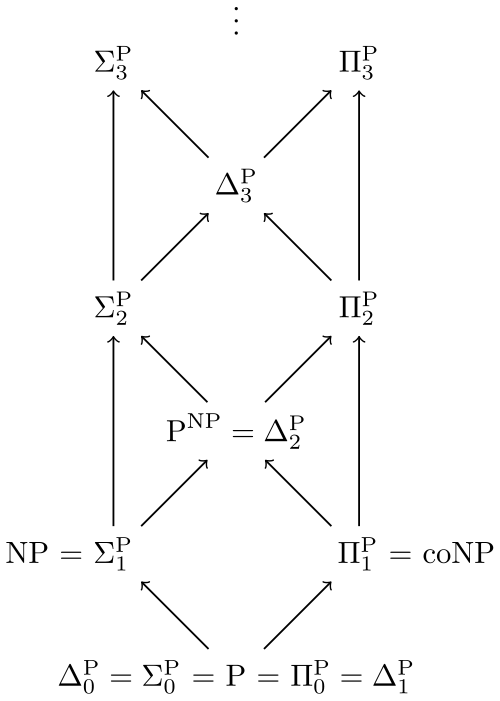
\includegraphics[width=0.3\textwidth]{img/ph_diagram.png}
  \caption{Polynomial hierarchy diagram \label{fig:ph_diagram}}
\end{figure}

\subsection{$\bPSPACE$}
In this work, we consider yet another complexity class called $\bPSPACE$ that
concerns the complexity of space.
It consists of problems that can be decided in polynomial space.

\begin{definition}
	The class $\bPSPACE$ is the class of decision problems solvable by a TM
	in space polynomial in the size of the input.
\end{definition}
It is not hard to see the following relation hold.
\begin{center}
	$\bPH \subseteq \bPSPACE$.
\end{center}

We illustrate the relationship among the complexity classes in
\figref{comp_diagram}. Many classes that are not in our focus 
are omitted from our diagram.

\begin{figure}[h!]
  \centering
  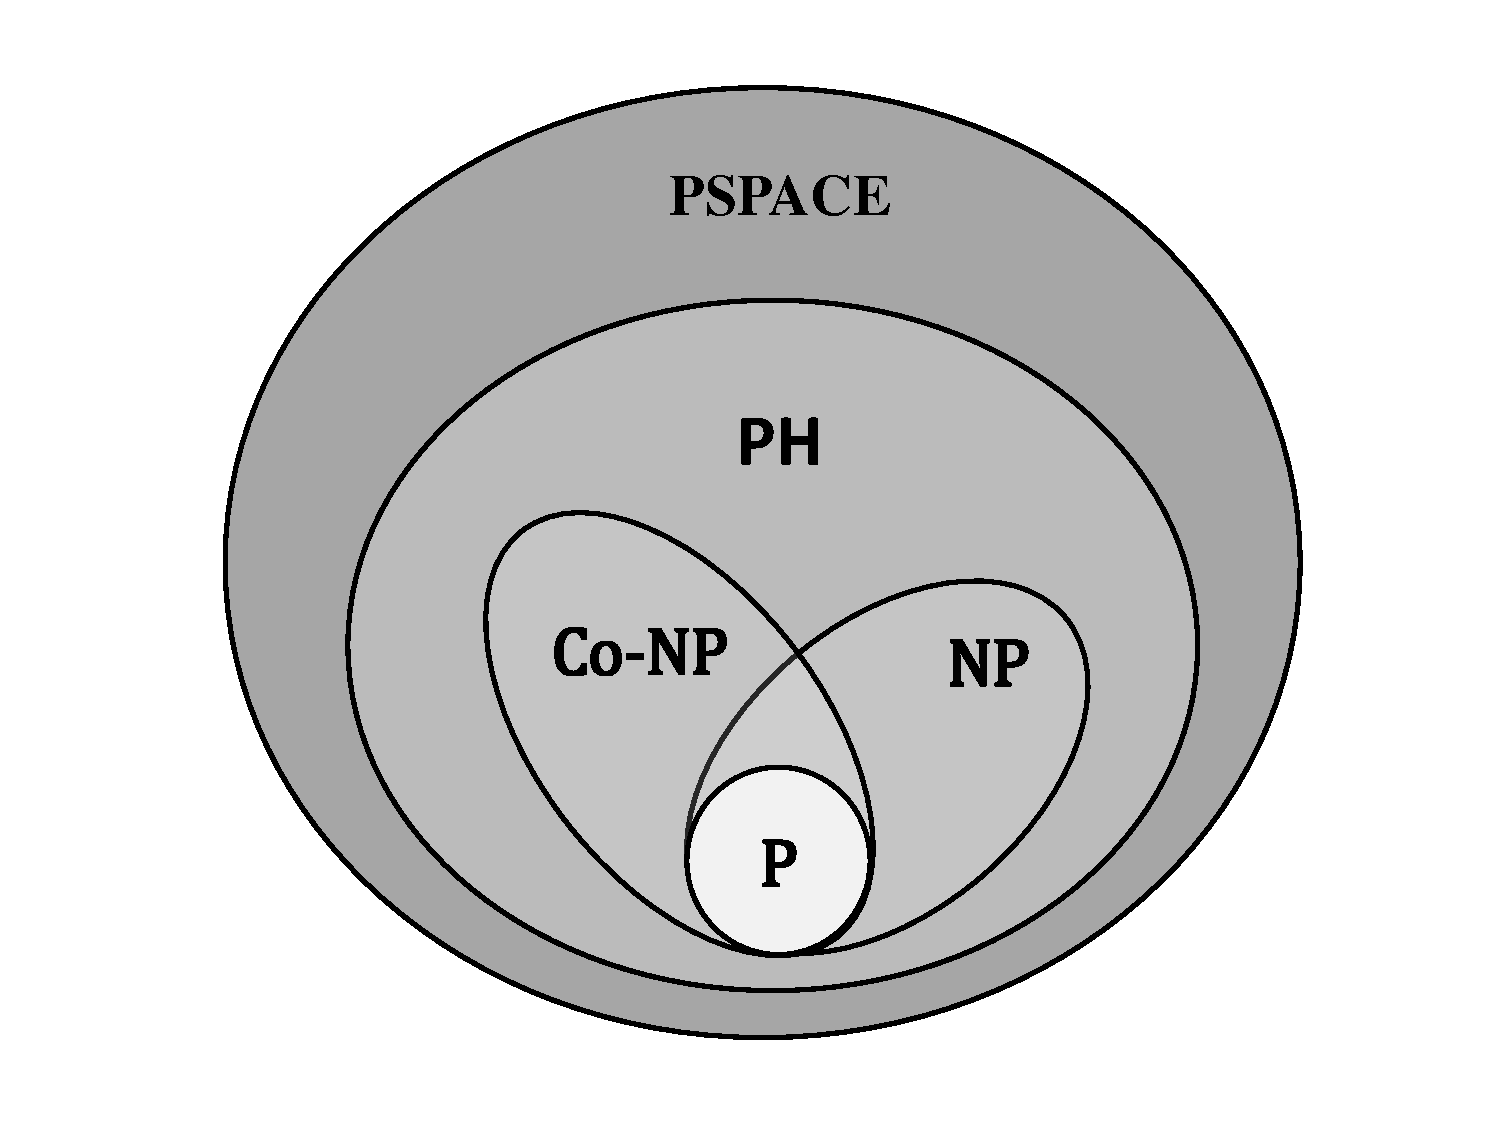
\includegraphics[width=0.7\textwidth]{img/comp_diagram.pdf}
  \caption{Computational complexity diagram \label{fig:comp_diagram}}
\end{figure}


